\section{Método Científico}


\begin{frame}
	\begin{block}{Qual o objetivo de uma equipe de dados?}
		 \begin{itemize}
			  \item Extrair valor dos dados!
			  \item O valor são: idéias, predições, padrões
			  \item Com esses insumos acima é possível para as empresas tomarem melhores decisões
		  \end{itemize}
	\end{block}
\end{frame}


\begin{frame}
	\begin{block}{Exercício}
		 \begin{itemize}
			  \item Como tomar melhores decisões?
		  \end{itemize}
	\end{block}
\end{frame}


\begin{frame}
	\begin{block}{Como tomar melhores decisões?}
		 \begin{itemize}
			  \item Usando dados e idéias obtidos anteriormente
			  \item Mas de que forma? Há um processo para isso?
		  \end{itemize}
	\end{block}
\end{frame}


\begin{frame}
	\begin{block}{Método Científico}
		 \begin{itemize}
			  \item É uma forma para extrair dados, analisar, criar hipóteses e tomar decisões
			  \item Evita que vc cometa erros comuns, não garante que não haverá erros
			  \item Citar exemplo do $6$ sigma ou outras normas de controle de qualidade.
		  \end{itemize}
	\end{block}
\end{frame}


\begin{frame}
	\begin{block}{Método Científico}
		 \begin{itemize}
			  \item Existe há  aproximadamente 300 anos nas áreas científicas
			  \item É um processo com passos para a validar uma determinada hipótese
			  \item Garante um determinado rigor no processo
			  \item É usado por cientistas do mundo inteiro para descobrir novos conhecimentos			  
		  \end{itemize}
	\end{block}
\end{frame}


\begin{frame}
	\begin{block}{Processo}
		\begin{figure}[!htb]
			\centering	  				
			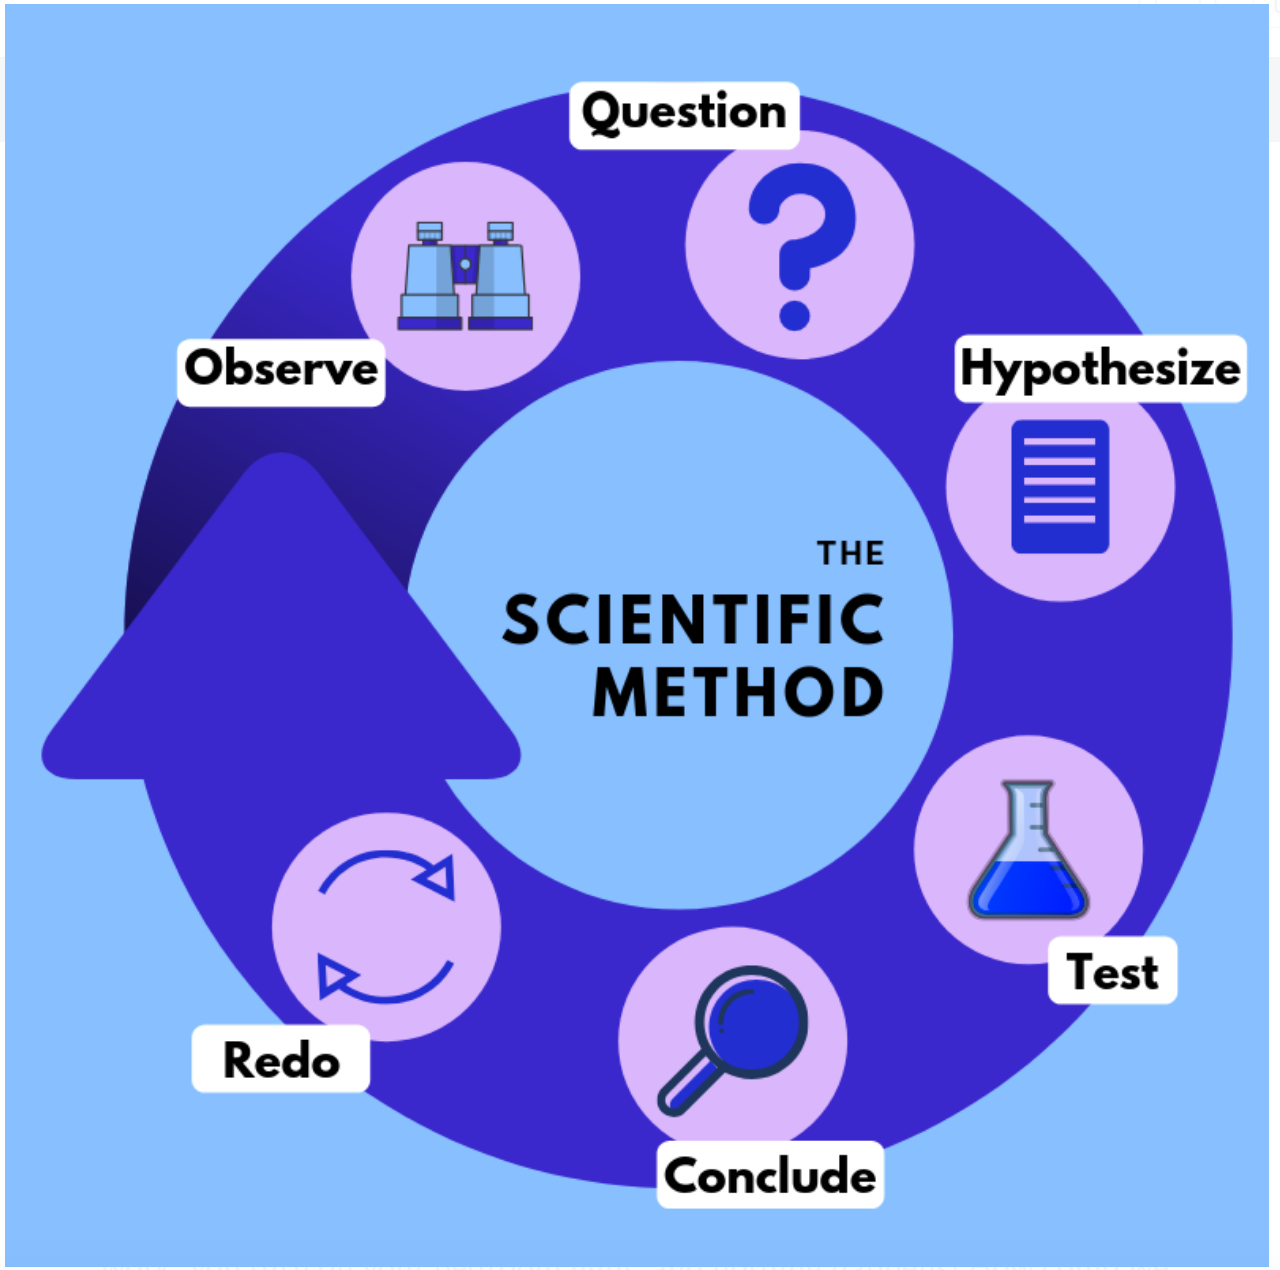
\includegraphics[height=5cm, width = 8cm]{./pic/metodoCientifico.png}
			\caption{Exemplo de método científico - processo}
		\end{figure}
	\end{block}
\end{frame}



\begin{frame}
	\begin{block}{Processo}
		  \begin{itemize}
			  \item  Observe: Queremos analisar algo... estudar algo... para tal, devemos observar esse evento. Tipicamente no mercado isso é um problema de negócio, no meio acadêmico um problema de pesquisa
			  
			  \item  Question: Após observar/estudar um problema inicial devemos elaborar hipóteses sobre ele. (O que são hipóteses?)

			  \item  Hypothesize: Uma pergunta/comportamento de negócio que queremos validar/explicar 

		  \end{itemize}
	\end{block}
\end{frame}


\begin{frame}
	\begin{block}{Processo}
		  \begin{itemize}

			  \item  Test: Devemos testar a hipótese e as possíveis predições, realizadas usando experimentos reproduzíveis

			  \item  Conclude: Analisar os resultados e tirar conclusões sobre eles, devemos validar a hipótese

			  \item  Redo: O experimento pode e deve ser refeito para garantir a consistência da teoria e validação da hipótese

		  \end{itemize}
	\end{block}
\end{frame}


\begin{frame}
	\begin{block}{Exemplo Simples}
		  \begin{itemize}

			  \item  Vamos supor que você tenta ligar a lâmpada de sua cozinha mas nada acontece (a luz não acende!)
			  
			  \item Como aplicar o método científico aqui?
			  
			  \item Podem descrever as etapas do processo?

		  \end{itemize}
	\end{block}
\end{frame}


\begin{frame}
	\begin{block}{Solução lâmpada}
		\begin{figure}[!htb]
			\centering	  				
			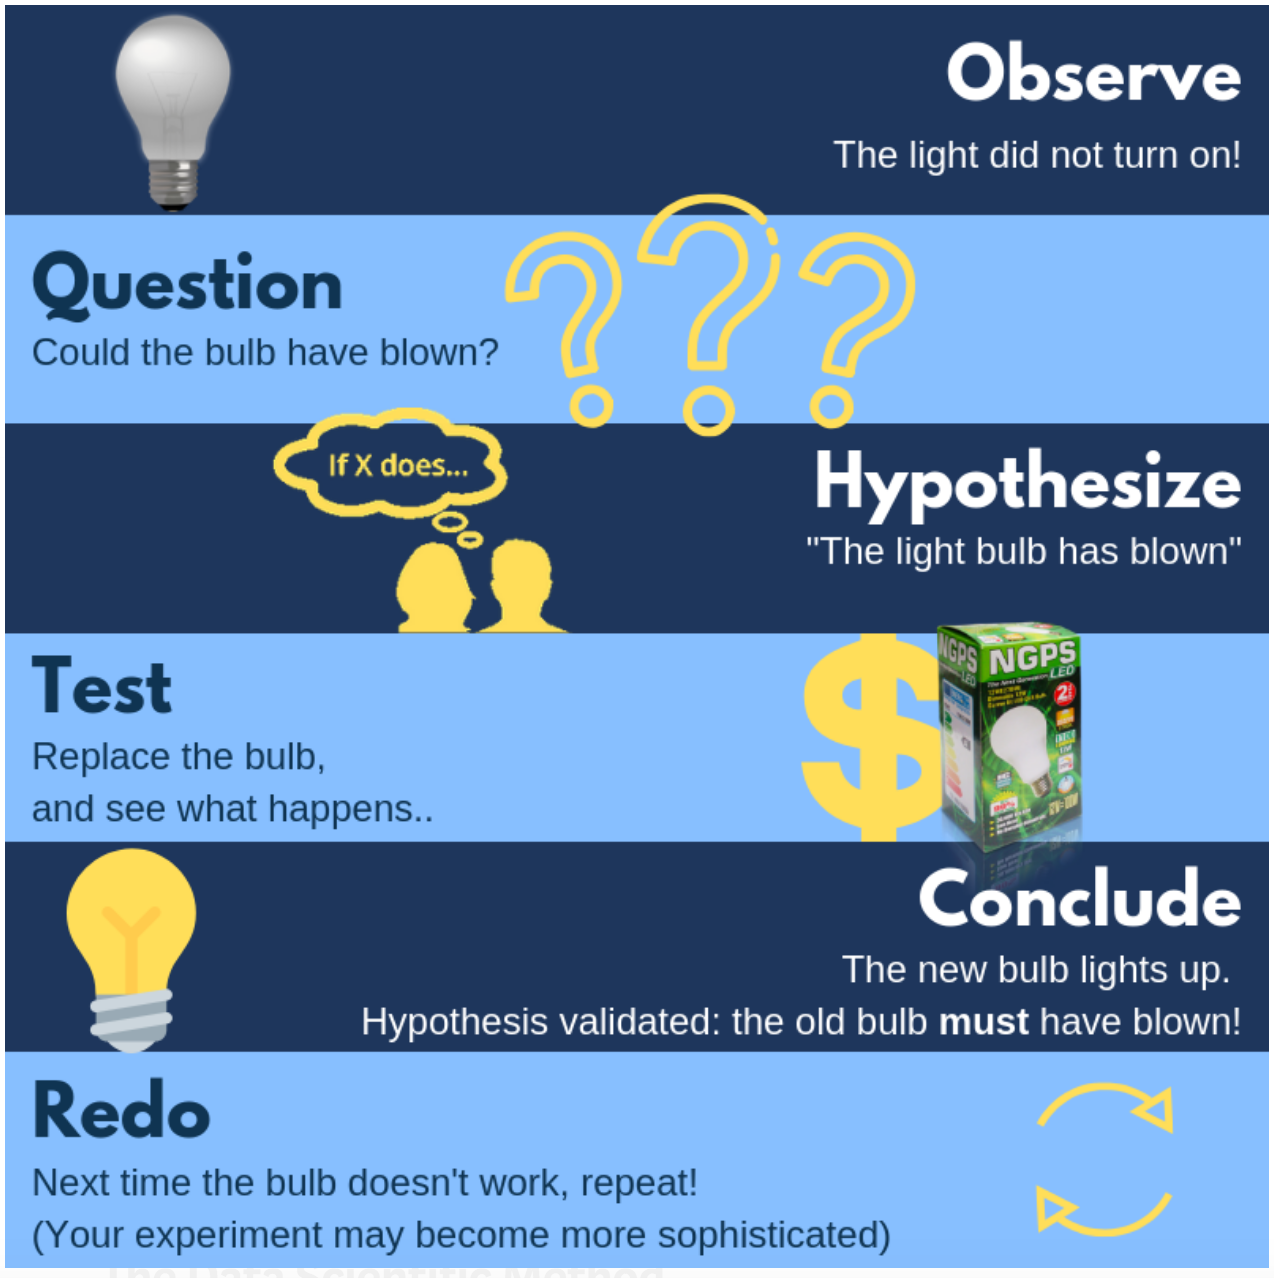
\includegraphics[height=5cm, width = 8cm]{./pic/exemploLampada.png}
			\caption{Solução lâmpada}
		\end{figure}
	\end{block}
\end{frame}



\begin{frame}
	\begin{block}{Exemplo Real}
		  \begin{itemize}

			  \item  Vamos supor que você trabalhe em uma área de análise de crédito de um banco.
			  
			  \item Como aplicar o método científico aqui?
			  
			  \item Podem descrever as etapas do processo?

		  \end{itemize}
	\end{block}
\end{frame}


\begin{frame}
	\begin{block}{Exemplo Real}
		  \begin{itemize}

			  \item Vamos supor que você trabalhe em uma área de análise de risco de transações de cartão de crédito.
			  
			  \item Como aplicar o método científico aqui?
			  
			  \item Podem descrever as etapas do processo?

		  \end{itemize}
	\end{block}
\end{frame}


\begin{frame}
	\begin{block}{Exemplo Real}
		  \begin{itemize}

			  \item Vamos supor que você trabalhe seja um médico.
			  
			  \item Como aplicar o método científico aqui?
			  
			  \item Podem descrever as etapas do processo?

		  \end{itemize}
	\end{block}
\end{frame}


\begin{frame}
	\begin{block}{Método Cinetífico}
		  \begin{itemize}

			  \item  A ciência estuda como aumentar o conhecimento da humanidade (óbviamente em áreas que não conhecemos ;) )
			  
			  \item Método científico é um método iterativo que padroniza o processo de conduzir experimentos, para ter resultados mais precisos, valiosos e confiáveis
			  
			  \item Para data science, IoT, podemos adaptar esse método para as empresas. Onde nosso objetivo é localizar informação de negócio.

		  \end{itemize}
	\end{block}
\end{frame}


\begin{frame}
	\begin{block}{Processo Adaptado}
		\begin{figure}[!htb]
			\centering	  				
			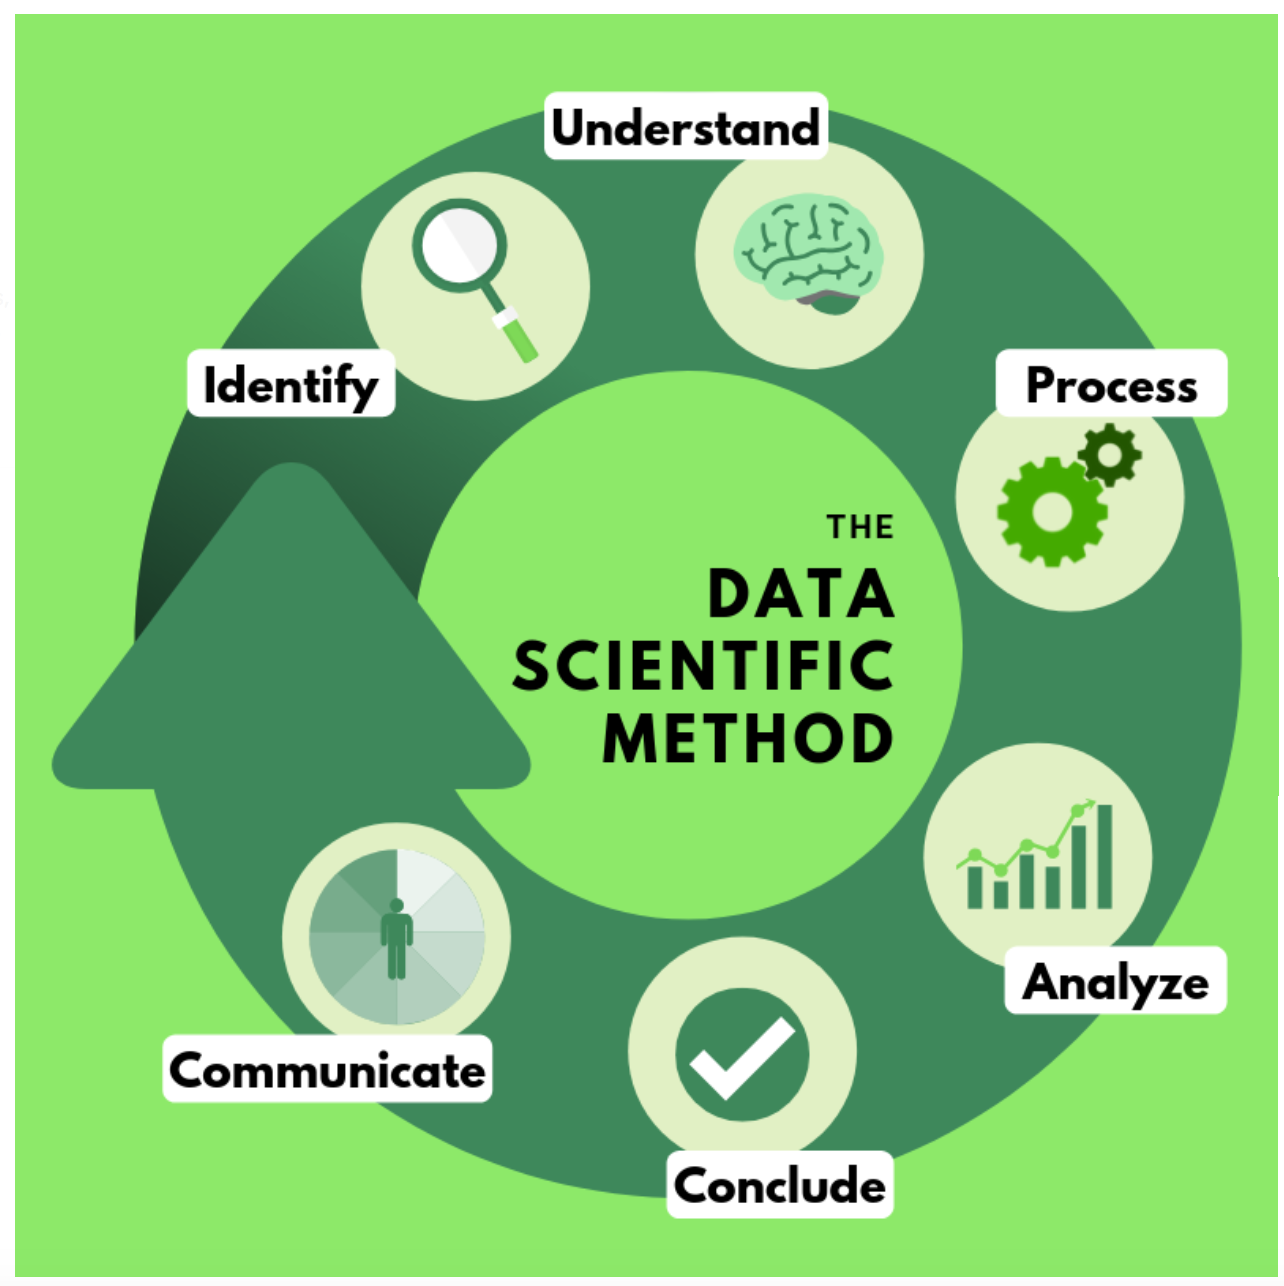
\includegraphics[height=5cm, width = 8cm]{./pic/metodoAdaptado.png}
			\caption{Exemplo de método científico - processo adaptado}
		\end{figure}
	\end{block}
\end{frame}


\begin{frame}
	\begin{block}{Processo Adaptado}
		\begin{itemize}

		\item Identificar: Nessa etapa identificamos a necessidade do negócio. 
		\item Que tipo de questões devemos responder?
		\begin{itemize}
			\item Que tipo de decisões devem ser tomadas com esses dados?
			\item Podemos formular hipóteses sobre esses dados? Quais?
			\item Quanto tempo temos para explorar?
			\item Quais decisões o cliente pretende tomar com esses dados?
			\item Qual seria o resultado ideal?
			\item Como apresentar os resultados?
		\end{itemize}		
			
		\end{itemize}								
	\end{block}
\end{frame}


\begin{frame}
	\begin{block}{Processo Adaptado}
	
		Ferramentas
		\begin{itemize}

			\item Entrevista com o cliente
			\item Brainstorm
			
		\end{itemize}								
	\end{block}
\end{frame}


\begin{frame}
	\begin{block}{Processo Adaptado}
		\begin{itemize}
		\item Entendimento: Ter um contato inicial com o conjunto de dados
		\item Que tipo de questões devemos responder?
			\begin{itemize}
				\item Tamanho dos dados? Linhas x colunas; Gb;..
				\item Quantos arquivos temos?
				\item Há quantas fontes de informação?
				\item Os dados de diferentes fontes tem formatação/tipagem igual?
				\item Necessita de limpeza?
				\item O que os campos (variáveis) significam?
				\item Há outliers?
				\item Há dados nulos?
			\end{itemize}
				
		\end{itemize}
	\end{block}
\end{frame}


\begin{frame}
	\begin{block}{Processo Adaptado}
	
		Ferramentas
		\begin{itemize}
			\item Workshops/brainstorming
			\item Jupyter Notebook
			\item Numpy and Pandas
			\item R
			\item seaborn/matplotlib
		\end{itemize}
	\end{block}
\end{frame}



\begin{frame}
	\begin{block}{Processo Adaptado}
		\begin{itemize}
		\item Processamento: Preparação dos dados, limpeza, padronização, tipagem, reshape de dados
		\item Que tipo de operações sobre os dados devemos realizar?
			\begin{itemize}
				\item Criar um dataset final para apresentar ao modelo
				\item Remoção de variáveis não úteis para o modelo (Como eu defino o que é ou não útil?)
				\item Remoção de duplicações
				\item Normalização
				\item Tipagem de dados deve ser unificada
				\item Decidir o que fazer com outliers
				\item Tratar dados null
			\end{itemize}
				
		\end{itemize}
	\end{block}
\end{frame}
    

\begin{frame}
	\begin{block}{Processo Adaptado}
	
		Ferramentas
		\begin{itemize}
			\item Workshops/brainstorming
			\item Jupyter Notebook
			\item Numpy and Pandas
			\item R
			\item seaborn/matplotlib
			\item NLTK (Natural Language Processing Toolkit — another Python library)
		\end{itemize}
	\end{block}
\end{frame}


\begin{frame}
	\begin{block}{Processo Adaptado}
		\begin{itemize}
		\item Análise: Estudos dos dados, entendimento de padrões, gráficos e relações.
		\item Aqui avaliamos valores de variáveis e suas distribuições, variáveis tomadas par a par, padrões sobre o tempo
		\item Validamos hipóteses definidas anteriormente, criamos modelos para predizer valores.
		\item Atividades típicas nesse estágio
				\begin{itemize}
					\item Se há dados temporais identificar sazonalidade e padrões no decorrer do tempo
					\item Se há dados geográficos identificar padrões espacias em conjunto com outras variáveis
					\item Correlação
					\item Variância
					\item Estatística descritiva (correlação, desvio padrão, box plot)
					\item Classificação de texto usando processamento de linguagem natural
					\item  Usar técnicas de machine learning (SVM, Redes Neurais, Xgboost, árvores, Random Forest)
					\item Técnicas de redução de dimensionalidade
				\end{itemize}		
		\end{itemize}
	\end{block}
\end{frame}
    

\begin{frame}
	\begin{block}{Processo Adaptado}
	
		Ferramentas
		\begin{itemize}
			\item Mysql/Postgresql/Cassandra/Mongo/Neo4J/Vertica/arquivos
			\item Jupyter Notebook
			\item JetBrains DataGrip (Pycharm IDE)
			\item R
			\item seaborn/matplotlib
			\item NLTK (Natural Language Processing Toolkit — another Python library)
			\item Scikit-Learn
			\item Tensor Flow
			\item Keras
		\end{itemize}
	\end{block}
\end{frame}

\begin{frame}
	\begin{block}{Inspiração}
		``If it disagrees with experiment, it’s wrong. In that simple statement is the key to science.'' — Richard P. Feynman
	\end{block}
\end{frame}



\begin{frame}
	\begin{block}{Processo Adaptado}
		\begin{itemize}
		\item Conclusões: Nessa fase devemos definir quais foram as conclusões que chegamos na fase de análise.
		\item Comprovamos as hipóteses?
		\item Quais planos de ação podemos definir?
		
				\begin{itemize}
					\item Validar se os achados permitem responder as questões originais
					\item Aceitar ou rejeitar hipóteses
					\item Definir as conclusões mais importantes para os clientes
					\item Descrever tudo em linguagem que o cliente possa entender
					\item Encontrar relações de pareto sobre os planos de ação
					\item Definir recomendações para o cliente					
				\end{itemize}		
		\end{itemize}
	\end{block}
\end{frame}

    
\begin{frame}
	\begin{block}{Processo Adaptado}
	
		Ferramentas
		\begin{itemize}
			\item Powerpoint
			\item Apresentação para o cliente
			\item Pareto
		\end{itemize}
	\end{block}
\end{frame}



\begin{frame}
	\begin{block}{Processo Adaptado}
		\begin{itemize}
		\item Comunicação: O cliente precisa te entender!
		\item Cliente não sabe o que é TCP/IP!
		\item Cliente quer resultados/informação e planos de ação para ganhar dinheiro
				\begin{itemize}
					\item Criar gráficos muito bonitos e simples para séries temporais (e.g. Grafana, Superset)
					\item Criar gráficos muito bonitos e simples para dados espaciais (e.g. Leaflet JS, Plotly ou Superset)
					\item Gráficos estatísticos (D3.js, Matplotlib or Seaborn)
					
				\end{itemize}		
		\end{itemize}
	\end{block}
\end{frame}

    
\begin{frame}
	\begin{block}{Processo Adaptado}
	
		Ferramentas
		\begin{itemize}
			\item Grafana
			\item Apache Superset
			\item Psycopg2
			\item Angular
			\item Microsoft Office
			\item D3.js
		\end{itemize}
	\end{block}
\end{frame}



\begin{frame}
	\begin{block}{Processo Adaptado}
		\begin{itemize}
			\item Plano de ação: Certo, o cliente entendeu.. mas ele está usando?		
				\begin{itemize}
					\item Se o cliente está usando ótimo... cso contrário o que podemos mudar?					
				\end{itemize}		
		\end{itemize}
	\end{block}
\end{frame}


\begin{frame}
	\begin{block}{Processo}
		\begin{figure}[!htb]
			\centering	  				
			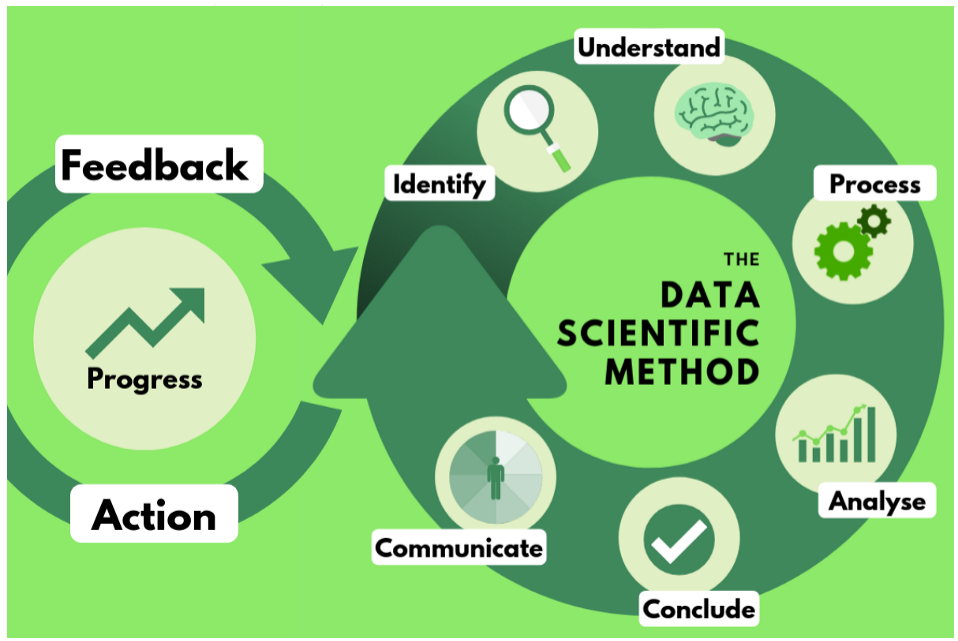
\includegraphics[height=5cm, width = 8cm]{./pic/metodoAdaptadoFeedback.png}
			\caption{Exemplo de método científico com feedback - processo}
		\end{figure}
	\end{block}
\end{frame}


\begin{frame}
	\begin{block}{Inspiração}
		``Without data, you’re just another person with an opinion.'' — W. Edwards Deming
	\end{block}
\end{frame}


\begin{frame}
	\begin{block}{Exercício}
		\begin{itemize}
			\item \href{https://www.kaggle.com/datasets}{\color{blue}{Kaggle}}
			\item \href{https://archive.ics.uci.edu/ml/index.php}{\color{blue}{UCI}} 
			\item Posso usar outro dataset? SIM ;)
		\end{itemize}
	\end{block}
\end{frame}
